%%%%%%%%%%%%%%%%%%%%%%%%%%%%%%%%%%%%%%%%%
% Journal Article
% LaTeX Template
% Version 1.4 (15/5/16)
%
% This template has been downloaded from:
% http://www.LaTeXTemplates.com
%
% Original author:
% Frits Wenneker (http://www.howtotex.com) with extensive modifications by
% Vel (vel@LaTeXTemplates.com)
%
% License:
% CC BY-NC-SA 3.0 (http://creativecommons.org/licenses/by-nc-sa/3.0/)
%
%%%%%%%%%%%%%%%%%%%%%%%%%%%%%%%%%%%%%%%%%

%----------------------------------------------------------------------------------------
%	PACKAGES AND OTHER DOCUMENT CONFIGURATIONS
%----------------------------------------------------------------------------------------

\documentclass[twoside,twocolumn]{article}

\usepackage{blindtext} % Package to generate dummy text throughout this template 
\usepackage[sc]{mathpazo} % Use the Palatino font
\usepackage[T1]{fontenc} % Use 8-bit encoding that has 256 glyphs
\linespread{1.05} % Line spacing - Palatino needs more space between lines
\usepackage{microtype} % Slightly tweak font spacing for aesthetics
\usepackage{epsfig}
\usepackage[english]{babel} % Language hyphenation and typographical rules
\usepackage{graphicx}
\usepackage[hmarginratio=1:1,top=32mm,columnsep=20pt]{geometry} % Document margins
\usepackage[hang, small,labelfont=bf,up,textfont=it,up]{caption} % Custom captions under/above floats in tables or figures
\usepackage{booktabs} % Horizontal rules in tables
\usepackage{amsmath}
\usepackage{lettrine} % The lettrine is the first enlarged letter at the beginning of the text
\usepackage{enumitem} % Customized lists
\setlist[itemize]{noitemsep} % Make itemize lists more compact

\usepackage{abstract} % Allows abstract customization
\renewcommand{\abstractnamefont}{\normalfont\bfseries} % Set the "Abstract" text to bold
\renewcommand{\abstracttextfont}{\normalfont\small\itshape} % Set the abstract itself to small italic text

\usepackage{titlesec} % Allows customization of titles
\titleformat{\section}[block]{\large\scshape\centering}{\thesection.}{1em}{} % Change the look of the section titles
\titleformat{\subsection}[block]{\large}{\thesubsection.}{1em}{} % Change the look of the section titles

\usepackage{fancyhdr} % Headers and footers
\pagestyle{fancy} % All pages have headers and footers
\fancyhead{} % Blank out the default header
\fancyfoot{} % Blank out the default footer
\fancyhead[C]{Graph Convolutional Network $\bullet$ December 2020 $\bullet$ Vol. XXI, No. 1} % Custom header text
\fancyfoot[RO,LE]{\thepage} % Custom footer text

\usepackage{titling} % Customizing the title section

\usepackage{hyperref} % For hyperlinks in the PDF

% Bibliography
% http://en.wikibooks.org/wiki/LaTeX/Bibliography_Management
%%%%%%%%%%%%%%%%%%%%%%%%%%%%%%%%%%%%%%%%%%%%%%%%
% Add the \citep{key} command which display a
% reference as [author, year]
\usepackage[backend=bibtex,
    bibencoding=utf8
]{biblatex}
\addbibresource{bib/mybib}
\usepackage{csquotes}
\usepackage[nottoc]{tocbibind}
\usepackage[toc,page]{appendix}


%----------------------------------------------------------------------------------------
%	TITLE SECTION
%----------------------------------------------------------------------------------------

\setlength{\droptitle}{-4\baselineskip} % Move the title up

\pretitle{\begin{center}\Huge\bfseries} % Article title formatting
\posttitle{\end{center}} % Article title closing formatting
\title{Exploring Recommender Systems with Graph Convolutional Networks} % Article title
\author{%
\textsc{Frederik Valdemar Schrøder, Jens Petur Tróndarson, Mathias Møller Lybech} \\[1ex] % Your name
\normalsize Aalborg University \\ % Your institution
\normalsize \href{mailto:fschra16@student.aau.dk}{fschra16@student.aau.dk} % Your email address
\normalsize \href{mailto:jtrand16@student.aau.dk}{jtrand16@student.aau.dk} % Your email address
\normalsize \href{mailto:mlybec16@student.aau.dk}{mlybec16@student.aau.dk} % Your email address
%\and % Uncomment if 2 authors are required, duplicate these 4 lines if more
%\textsc{Jane Smith}\thanks{Corresponding author} \\[1ex] % Second author's name
%\normalsize University of Utah \\ % Second author's institution
%\normalsize \href{mailto:jane@smith.com}{jane@smith.com} % Second author's email address
}
\date{\today} % Leave empty to omit a date
\renewcommand{\maketitlehookd}{%
\begin{abstract}
\noindent  
Graph Convolutional Network (GCN) is a state-of-the-art method for collaborative filtering (CF).
Throughout this paper we focus on two new methods for CF: LightGCN and Price-aware Recommendation with Graph Convolutional Networks (PUP).
LightGCN is inspired from Neural Graph collaborative Filtering (NGCF), and is a recommender system that only take the node ID of item and users into account.
PUP also utilize CF, but takes prices and categories into account. 
We take a closer look at the main differences between LightGCN, NGCF and PUP.
After we have found the main differences between these, we extend LightGCN and NGCF by adding prices and categories as nodes in their input graph.
Through our experiments we show that our extension was unsuccesfull in improving the performance of these methods.
In our experiments we run our extension with different hyper parameters to see what effect they have on the results.
We also compare LightGCN to some other state-of-the-art methods and show that it performs significantly better than PUP, NGCF and the other methods.
From the results of these experiments we present some reasons to why our extension performed so poorly.
We end the paper by presenting some possible hypotheses that we can continue to work on in our master thesis.
\end{abstract}
}

%----------------------------------------------------------------------------------------
\lstset{
	basicstyle=\footnotesize,
	numbers=left, 
	numberstyle=\tiny, 
	framexleftmargin=0pt,
	breaklines=true,
	tabsize=2
}

\begin{document}

% Print the title
\maketitle

%----------------------------------------------------------------------------------------
%	ARTICLE CONTENTS
%----------------------------------------------------------------------------------------

\section{Introduction}
Recommendation systems are widely being used to help users browsing on the internet attenuate information overload\cite{YT_rec,Pint_rec}.
The general idea behind a recommendation system is to predict whether a user will interact with a given item, e.g. purchase, rate, watch, based upon their historical data with similar items.
Collaborative filtering (CF) tackles this problem by assuming that users can be used by the recommendation system to recommed items for other users who have similar preferences on items.
Generally, the most common way to achieve this is to firstly learn latent features to represent a user and an item, this process is also called embedding.
Secondly the embeddings are used for performing predictions.
\\
An early model for CF is Matrix Factorization, which embeds user and item ID as vectors and uses the dot product to predict whether a user would like a certain item.
Though MF models have shown to perform quite well, \cite{NGCF_2019} proposes Neural Graph Collaborative Filtering (NGCF).
\\ 
NGCF argues that earlier models do not integrate the user-item interactions especially the bipartite graph structure in their embeddings.
Therefore missing out on collaborative signals which could aid in recommendation.
By utilizing a Graph Convolutional Network (GCN) they are able to achieve great performance compared to other baselines.
\\
GCN's has become the new state-of-the-art for CF but the reason for their effectiveness is not fully understood\cite{lightgcn}.
Through empirical testing, \cite{lightgcn} shows that feature transformation and nonlinear activation, the two most common designs in GCN's, do very little to contribute to more accurate predictions.
They then go on to propose a simple implementation of GCN called LightGCN which achieves even better performance than its more complex GCN counterparts.
\\
Looking at papers such as \cite{Priceaware} it can be seen that propagating the influence of price on users with items as a bridge, as well as integrating category into the propagation progress increases the performance.
Since \cite{Priceaware} also utilizes a GCN our idea is to improve the performance of the LightGCN framework by utilizing price and category.

\section{Basic Theory}

\subsection{Graph Convolutional Network}
Graph Convolutional Network (GCN) is a neural network architecture that operates on graphs.
Given a graph $G = (V,E)$ a GCN takes the input of a adjacency
matrix $A$ with size of $N x N$ that represents graph $G$ and a feature matrix $N x F^0$, where $N$ is the total amount of nodes and $F^0$ is the total amount of input features for each node.\\
\indent
A hidden layer in a GCN can be defined as $H^i = f(H^{i-1}, A)$ where $i$ indicates the layer and $H^0$ is the previously mentioned $N x F^0$ feature matrix and $f$ is a propagation function \cite{Deep-Learning-on-Graphs-with-GCN}.
There are many different types of propagation functions.
A simple example could be $f(H^i, A) = \sigma(AH^iW^i) = H^{i+1}$ where $W^i$ is the weight matrix at layer $i$ and $\sigma$ is a non-linear activation function \cite{Deep-Learning-on-Graphs-with-GCN}.
The intuition behind this propagation function is that the future representation of each node is calculated based on its neighbors nodes.
Each time $i$ is increased, the nodes will reach one further edge away from the original node in the graph. %Fuck this sentence
An issue with this propagation function could be that the value of each node now is a sum of each of its neighbors, and therefore loses its own value.
This could be solved by replacing $A$ with $\hat{A} = A + I$ where $I$ is the identity matrix.
Doing this the node considers itself a neighbor.

\section{Related work}
In this section we take a look at existing work that relates to what we have studied to acquire the knowledge to extend Light GCN model.

\subsection{Collaborative Filtering}
Collaborative Filtering (CF) is one of the most prevalent techniques in current recommendation systems\cite{YT_rec,NGCF_2019,Pint_rec,COL_MEM_NET}.
One of the most common ways to achieve CF is by parameterize users and items as embeddings and afterwards learn the embedding parameters by reconstructing historical user-item interaction from these embeddings\cite{NGCF_2019}
One of the earliest CF models were Matrix Factorization (MF) \cite{Matrix-factorization-techniques, BAY_PER_RAN}.
MF  projects the ID of each user and item into embedding vectors and uses the dot product between them to predict an user-item interaction.
While the dot product can be used to predict user-item interaction its linearity makes it unable to capture more complex relationships between users and items.
Newer more sophisticated techniques utilize neural networks to enhance the interaction modeling while keeping the same embedding as the older MF models.
Some examples of this are the NMF model\cite{NEU_COL_FIL} which uses nonlinear neural networks as its interaction function and the LRML model\cite{LAT_REL_MET} which utilizes Euclidean distance metrics to model the interaction strength.
Other approaches include trying to improve the embedding function.
To do this a lot of effort has been done to take side information into account such as item content\cite{ATT_COL_FIL_MUL}, social relations\cite{REC_SOC_USE} and external knowledge graphs\cite{KGAT, KNO_GRA_REC}.
Other methods use the weighted average of the ID embeddings of historical items as the pre-existing features of a user and thereby improving the user representation\cite{SVD_PLUSPLUS,FISM}.
 
\subsection{Graph-Based Recommendation}
Another interesting technique is to look at the user-item graph structure and exploit it for better performance in recommendation systems.
Some of the earlier methods uses label propagation such as ItemRank\cite{ItemRank} and BiRank\cite{BiRank}.
To get the score of items for a specific user these methods define the labels as the users interacted items and propagate the labels on the graph ie. engouraging connected nodes to have similiar labels.
These methods lack model parameters and are therefore not able to properply optimize the objective function\cite{NGCF_2019}.
To work around this problem methods like HOP-Rec \cite{HOP_Rec} was created.
HOP-Rec combines graph based and embedding based methods and performs random walks to enrich the interactions of a user with multi-hop connected items.
HOP-Rec's better performance compared to MF models indicates that utilizing the connectivity information provides better embeddings.
Graph Neural Networks (GNN) provides new ideas on how to model graph structure to guide the embedding learning.
One such approach is GraphSAGE\cite{IND_REP_LEA} which aggregates feture information from a node's neighboorhood e.g. degrees or text attributes.
Because of the strengths related to graph convolution a lot of effort has went into creating recommendation systems\cite{NGCF_2019,GC_MC,Priceaware}, utilizing GCN on the user-item interaction graph to better capture CF signals in high-hop neighboors.
But Wu et al. \cite{SGCN} argues that GCN is unnecessaryily complex and proposes a simplified linear model they call Simple Graph Convolution that removes the nonlinearity of GCN and merges multiple weights into one.
Based on this article and others \cite{PRE_PROP,DEEP_GCN}, HE et al. \cite{lightgcn} proposes LightGCN.
LightGCN and SGC seems similiar but SGC is for node classification and simplifies GCN for efficiency and interpretability, while LightGCN is for CF.
nonlinearity and weight matrices are not usefull for CF and makes model training less effective.

\section{Method}

\subsection{Generated adjacency matrix}
In the following subsection the generated adjacency matrices of LightGCN and price aware recommendation are described.
Both use the adjacency matrix as a representation for a heterogeneous graph, where the value 1 represent a connection between two nodes.

\subsection{LightGCN}
For LightGCN the adjacency matrix is the size of $\textrm{number of users} + \textrm{number of items} \times \textrm{number of users} + \textrm{number of items}$.
Then for every connection between item $i$ and user $u$ 1 is inserted.
It is generated with SciPy that creates a dictionary of keys, where two keys indicate the position in the matrix, and the value is 1 if there is a connection. 
As users are unable to have a connection with other users, and the same with items, they are able to exploit this by inserting all connections from users to items, and then transposing the matrix.

\subsection{Price-aware recommendation}
The adjacency matrix in price-aware recommendation is also implemented as a sparse matrix using SciPy.
This is done by creating two arrays, row and column.
The row and column are both the length of all interactions plus two times the amount of items.
We start by for each user inserting their id as many times to the array as the number of items that they have interacted with.
The id's of the items that the user interacted with are mapped to the corresponding index in the column array.
After all user item interactions have been mapped to the row and column arrays, the item prices and category relationships are mapped to the arrays.
This is done by inserting the index of an item into the row twice.
At the indexes where the item was added to the row, the corresponding category and price related to that item are inserted to the column.
A third array is created with the length of row where ones are inserted.
Using this array, column and row can create a sparse adjacency matrix by mapping the index $i$ in row and column to the array with ones.
Within the adjacency matrix, there will be inserted 1 if there is a connection between item $i$ and user $u$, item $i$ and category $c$, and item $i$ and price $p$.
This results in a adjacency matrix that is of size number of users + number of items + number of categories + number of prices $\times$ number of users + number of items + number of categories + number of prices.

\subsection{Embeddings comparison}
In the following subsections the embeddings of LightGCN, NGCF and Price-aware recommendation are described.
Unlike with the adjacency matrices, the difference between the embeddings of NGCF and LightGCN are significant here.
For all nodes including categories and prices, the only value used is the node ID.
They utilize the embedding layer to compress the one-hot ID encoding to embeddings, so that each node has a separate embedding $e' \in \mathbb{R}^d$, where $d$ is the dimension size.

\subsubsection{LightGCN}\label{subsubsec:lightgcn-embedding}
The embeddings for LightGCN are constructed as follows \cite{lightgcn},
\begin{equation}
    E^{(k+1)} = (D^{\frac{1}{2}}AD^{\frac{1}{2}}E^{(k)}),
\end{equation}
where $A$ is the adjacency matrix containing users and items (described in \autoref{subsubsec:lightGCN-adj}) and $D$ is a diagonal matrix, where $D_{ii}$ denotes the sum of the $i-th$ row in the adjacency matrix $A$.
The $0th$ layer embedding is initialized as random normalized values, where $E^{(0)} \in R^{(I + U)\times T}$, and $T$ is the embedding size.
The final embedding is obtained as follows,

\begin{equation}
    e_u = \sum_{k=0}^{K} \alpha_k e_u^{(k)};\;\;\; e_i = \sum_{k=0}^{K} \alpha_k e_i^{(k)},
\end{equation}
where $\alpha$ is set to $1/(K + 1)$ and is used to normalize the embeddings.
$K$ is the number of layers defined, and $k$ is the current layer.

\subsubsection{NGCF}\label{subsubsec:NGCF-embed}
The embeddings for NGCF are constructed as follows \cite{NGCF_2019},
\begin{equation}
    \begin{split}
        E^{(l)} = &LeakyReLU((\lambda + I)E^{(l-1)}W_1^{(l)}+\\
        & \lambda E^{(l-1)}\bigodot E^{(l-1)}W_2^{(l))},
    \end{split}
\end{equation}
where $E^{(l)} \in \mathbb{R}^{I+U \times T}$ are the item and user embeddings after $l$ convolutions.
$E^{(0)} \in \mathbb{R}^{I+U \times T}$ is the $0th$ layer embedding, where $T$ is the embedding size.
$I$ is the identity matrix.
$W_1^{(l)}$ and $W_2^{(l)}$ are trainable weight matrices.
$\lambda$ is the Laplacian matrix for the user-item, item-price and item-category graph, and is defined as follows:
\begin{equation}
    \lambda = D^{\frac{1}{2}}AD^{\frac{1}{2}},
\end{equation}
where $A$ and $D$ are the adjacency and diagonal matrix.

\subsubsection{Price-aware recommendation}\label{subsubsec:price}
The input parameters when constructing the embeddings are the adjacency matrix $A \in \mathbb{R}^{N \times N}$ and identity matrix $I \in \mathbb{R}^{N \times N}$, where $N$ is the number of nodes.
Embeddings from node j to node i are propagated as follows \cite{Priceaware},
\begin{equation}
    t_{ji} = \frac{1}{|\mathcal{N}_i|}e'_j,
\end{equation}
where $\mathcal{N}_i$ is the set of neighbors for node $i$ and $e'_j$ is the embedding node j.
The updating rule is,
\begin{equation}
    \begin{split}
        & o_u = \sum_{j \in \{i \textrm{ with } R_{ui}=1 \} \cup \{ u\}}^{} t_{ju}                            \\
        & o_i = \sum_{j \in \{u \textrm{ with } R_{ui}=1 \} \cup \{ i, \textbf{c}_i \textbf{p}_i\}}^{} t_{ji} \\
        & o_c = \sum_{j \in \{i \textrm{ with } \textbf{c}_i=c \} \cup \{ c\}}^{} t_{jc}                      \\
        & o_p = \sum_{j \in \{i \textrm{ with } \textbf{p}_i=c \} \cup \{ p\}}^{} t_{jp}                      \\
        & e_f = \textrm{tanh}(o_f), f \in \{u, i, c, p\},
    \end{split}
\end{equation}
where $e_u$, $e_i$, $e_c$, and $e_p$ are the embeddings for user $u$, item $i$, category $c$ and price $p$ respectively.
These embeddings are used to compute the predictions as described in \autoref{subsec:price-intro}.

\subsubsection{Differences in embeddings}
The difference between NGCF and LightGCN are that NGCF utilizes the $LeakyReLU$ activation function as well as using the trainable weight matrices.
While NGCF and LightGCN are constructed for collaborative filtering without additional side information, the construction of the embeddings in Price-Aware recommendation focuses on constructing additional embeddings for both price and category, and utilizing these to compute predictions.


\subsection{Simple price aware extension of LightGCN}\label{subsec:simple-extension}
\begin{figure}
    \centering
    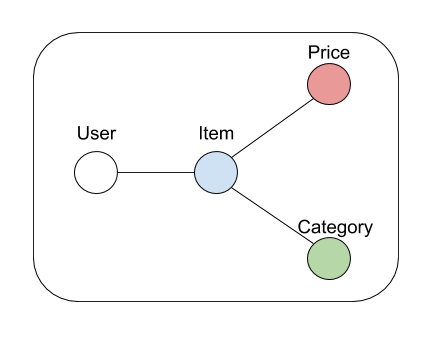
\includegraphics[scale=0.5]{figures/uipc.png}
    \caption{Illustration of the nodes in the simple extension of LightGCN.}
    \label{fig:uipc}
\end{figure}
We try to extend the implementation of LightGCN by changing the input parameters, where we construct the adjacency matrix containing the users, item, category and price graph, which is illustrated in \autoref{fig:uipc}.
The intuition behind the idea, is that the graph convolutions will capture the values of categories and price, so even if we do not use the embeddings for price and category, they will still influence users and items.
Let the user-item, item-price and item-category interactions matrix be $R \in \mathbb{R}^{I \times U + C + P}$, where $I$ denotes the number of items, $U, C, P$ denotes the number of users, categories and prices.
Each entry of $R_{ui}$ is 1 if user $u$ has rated item $i$. Otherwise it is 0.
If there is a connection in $R_{ic}$ or $R_{ip}$ this value is a hyperparameter $X$ with a value $x>0$, otherwise it is 0.
The adjacency matrix is obtained as follows:
\begin{gather}
    A =
    \begin{bmatrix}
        0   & R \\
        R^T & 0
    \end{bmatrix}
\end{gather}
The embeddings for users and price are calculated as follows,
\begin{equation}
    E^{(k+1)} = D^{\frac{1}{2}}AD^{\frac{1}{2}}E^{(k)},
\end{equation}
where $A$ is the adjacency matrix containing users, items, categories and price, and $D$ is a $(I + U + C + P)$ diagonal matrix, where $D_{ii}$ denotes the sum of the $ith$ row in the adjacency matrix $A$.
The $0th$ layer embedding $E^{(0)} \in R^{(I + U + C + P)\times T}$, where $T$ is the embedding size.
We do not change anything else in LightGCN in this method.

\subsection{Simple price aware extension of NGCF}
To gain an understanding of the effect of feature transformation and nonlinear activation function a price aware extension has also been added to NGCF.
The adjacency matrix is constructed as described in \autoref{subsec:simple-extension}.
The embeddings for user and price are calculated as follows,

\section{Experiment}
\subsection{Equal data} \label{equal-data}
When measuring the performance of the different methods it is essential that the datasets are the same.
Without them being equal the results of the experiments wont be worth comparing.
Both PUP and LightGCN utilized the yelp dataset according to their papers.
We did not get the dataset from the PUP implementation and were unable to find the original yelp-2018 dataset from the LightGCN implementation where the price and category were still attached.
We therefore decided to utilize the yelp-2020 dataset, in which users rank businesses between 1 to 5 stars.
Inspired by the PUP method we also decided to only use businesses with the restaurant category.
What is left is a set of businesses with one or more subcategories that relate to what type of restaurant they are.
Like PUP we cut off any extra subcategories so that each business now only has one subcategory.
The single subcategory that an item possesses is referred to as its category in the rest of this paper.
\\
PUP has a 60\% training-, 20\% validation- and 20\% test-data split while LightGCN has a 70\% training-, 10\% validation-, and 20\% test-data split.
It was decided to use the LightGCN split since this was the method we planned to extend.
\\
After this, we now have a dataset that can be used to compare the different methods with or without category and price.

\subsection{Experimental Settings}
\subsubsection{Evaluation metrics}
The evaluation metrics for rating top k recommendation, we utilize recall@K and ndcg@K where K is set to 50 and 100.
For all tests, the number of convolutions are set to 3.

\subsubsection{Baselines}
The following methods are used to compare the results from our experiment with.
\begin{itemize}
    \item \textbf{PUP} \cite{Priceaware}: PUP utilizes price and categories to improve the recommendation performance with Graph Convolutional Networks. A more detailed description of PUP can be seen in \autoref{subsec:price-intro}.
    \item \textbf{NGCF} \cite{NGCF_2019}: NGCF utilizes an embedding propagation layer and Graph Convolutional Network. It was created with the purpose of collaborative filtering. More details can be seen in \autoref{subsec:lightgcn-ngcf}.
    \item \textbf{LightGCN} \cite{lightgcn}: LightGCN was created from NGCF and showed improved results in training and NDCG by removing feature transformations and nonlinear activation function. More details can be seen in \autoref{subsec:lightgcn-ngcf}.
    \item \textbf{GCN} \cite{kipf2017semisupervised}: GCN is used for semi-supervised classification on graphs.
    \item \textbf{GC-MC} \cite{berg2017graph}: GC-MC utilizes Graph Convolutional Networks to create the representations for users and items. It only takes the first-order neighbor into account, and therefore only uses one convolution layer.
\end{itemize}
\subsection{Performance comparisons}
As can be seen on \autoref{tab:results-with-many-methods} LightGCN outperforms all the other methods by a significant amount.
With our dataset NGCF performs better than PUP by a small amount, even though Price-Aware recommendation in their paper showcased the opposite \cite{Priceaware}.
Price-Aware recommendation also uses a Yelp dataset for their experiment, however it is not exactly the same dataset.
The results also showcase, that there are a large decrease in performance, when adding prices and categories to the adjacency matrix in LightGCN, which makes it perform worse than any other baseline method.
For NGCF PAS the same changes in input only makes it differentiate negatively by a small amount and actually performs better than PUP.

\begin{table*}[h!]
    \centering
    \begin{tabular}{|l|l|l|l|l|}
        \hline
        \rowcolor[HTML]{FFFFFF}
                       & \multicolumn{4}{l|}{\cellcolor[HTML]{FFFFFF}Yelp Dataset}                                                       \\ \hline
        Method         & Recall@50                                                 & NDCG@50         & Recall@100      & NDCG@100        \\ \hline
        LightGCN       & \textbf{0.2106}                                           & \textbf{0.1063} & \textbf{0.3176} & \textbf{0.1344} \\ \hline
        PUP            & 0.1697                                                    & 0.07802         & 0.2654          & 0.1023          \\ \hline
        GCN            & 0.1558                                                    & 0.07593         & 0.2442          & 0.1001          \\ \hline
        NGCF           & 0.1810                                                    & 0.08817         & 0.2769          & 0.1132          \\ \hline
        GCMC           & 0.1692                                                    & 0.0835          & 0.2497          & 0.1008          \\ \hline
        LGCN PAS (1.0) & 0.1542                                                    & 0.0717          & 0.2199          & 0.086           \\ \hline
        NGCF PAS (1.0) & 0.1749                                                    & 0.0849          & 0.2743          & 0.1111          \\ \hline
    \end{tabular}
    \caption{Results for the experiment with the different methods}
    \label{tab:results-with-many-methods}
\end{table*}

\subsubsection{Hyperparameter experiment}
As described in \autoref{subsec:simple-extension}, we utilize a hyperparameter that is inserted into the adjacency matrix, whenever there is a connection between the item nodes and category nodes, or item nodes and price nodes.
The hyperparameter $X$ in LGCN PAS and NGCF PAS is tested with the values of $0.0$, $0.5$, $1.0$ and $2.0$ to see the effect of this as input data has on the final result.
\begin{table*}[h!]
    \centering
    \begin{tabular}{|l|l|l|l|l|}
        \hline
        \rowcolor[HTML]{FFFFFF}
                       & \multicolumn{4}{l|}{\cellcolor[HTML]{FFFFFF}Yelp Dataset}                                   \\ \hline
        Method         & Recall@50                                                 & NDCG@50 & Recall@100 & NDCG@100 \\ \hline
        LGCN PAS (0.0) & 0.1560                                                    & 0.07674 & 0.2456     & 0.09901  \\ \hline
        LGCN PAS (0.5) & 0.1591                                                    & 0.07825 & 0.2539     & 0.1010   \\ \hline
        LGCN PAS (1.0) & 0.1542                                                    & 0.0717  & 0.2199     & 0.086    \\ \hline
        LGCN PAS (2.0) & 0.1526                                                    & 0.07573 & 0.1581     & 0.06509  \\ \hline
        NGCF PAS (0.0) & 0.1758                                                    & 0.08483 & 0.2737     & 0.1111   \\ \hline
        NGCF PAS (0.5) & 0.1756                                                    & 0.08472 & 0.2744     & 0.1108   \\ \hline
        NGCF PAS (1.0) & 0.1749                                                    & 0.08485 & 0.2743     & 0.1111   \\ \hline
        NGCF PAS (2.0) & 0.1741                                                    & 0.08371 & 0.2762     & 0.1116   \\ \hline
    \end{tabular}
    \caption{Results for the experiment using different input values.}
    \label{tab:hyperparameter-results}
\end{table*}
As can be seen on \autoref{tab:hyperparameter-results} inserting categories and price into the adjacency matrix decreases the performance compared to LightGCN.
The value it performs best with is 0.5, followed by 0.0.
Giving prices and categories the same or higher input value as the connection between item and user therefore decreases the results.
There could be multiple reasons for this generally not performing well.
The embeddings created from this input could be used, so that it tries to recommend prices and categories, which is not possible.
Another reason could be because LightGCN does not utilize feature transformation and the nonlinear activation function.
LightGCN performs well, if there are only user and item ids, and the decrease in performance could be because LightGCN is unable to handle the semantic representations in price and category.\\
For NGCF changing the input value of price and categories changes almost nothing.
This is likely because the embeddings for price and categories are never used.
However, we did have an initial idea, that the convolutions with price and category would be reflected onto users and items, which is seen to give a very minimal effect on the outcome.


\section{Discussion}
\section{Future work}\label{sec:future-work}
For our master thesis, we will continue to explore recommendation systems and continue in the path of LightGCN and PUP.
There are several topics related to these implementations to be investigated to gain a better understanding of how recommender systems can be improved.
The hypotheses for the master thesis are:
\begin{itemize}
    \item Adding price and category embeddings to LightGCN will improve the performance of the simple PUP extension.
    \item If adding price and category embeddings improves the performances, then it can get generalized to include other features than price and category.
    \item PUP can be generalized so other features can get integrated to improve the recommendation performance.
    \item Extending categories so one item can have multiple categories will better capture cross-category price preferences.
\end{itemize}

\subsection{Adding PUP embeddings to LightGCN}
An extension of the embeddings in LightGCN could be implemented by combining the embeddings from the different methods.
Inspired by utilizing \autoref{eq:price-aware-prediction}, we could use the embeddings for price and category.
An alternative could be trying to combine the original LightGCN embedding without price and category for users and items, as these capture the collaborative filtering quite well and then adding the price and category embeddings.
A possible outcome of this can however be that there still are contradictions between the collaborative signals, and price and category signals.
LightGCN does not utilize feature transformation and non-linear activation functions, which can make it not suited for handling side information.
PUP and NGCF do use feature transformation and non-linear activation functions, so if extending LightGCN is not feasible, we should be able to do it with NGCF.

\subsection{Generalizing feature inputs for LightGCN or PUP}
The intuition behind PUP can be used for other datasets with other types of data.
Before it would make sense to generalize the feature inputs in the adapted LightGCN, we would first have to make sure that adding the price and category was actually beneficial for the method.
If extending LightGCN is not feasible, then NGCF could be extended, as this has shown interesting results.
An example could be if we try to recommend movies to users, then instead of price and category, these could be replaced with actors or genre, or other types of data.
For prices and categories, a user can have different preferences for the price range in different categories.
The same can be applied for actors in movies, where users could prefer different actors in different genres, but these might not be as related as prices and categories.
Therefore we would need to experiment with different graphs, where users could be connected to items, genres, or actors, or where the item is a bridge between genres, actors, and users.

\subsection{Extending categories}
To prove their concept PUP decided to only retain one category for each item even though the dataset used has multiple categories for each item.
Having multiple categories might help to better capture cross-category price preferences.
It might also increase noise by having too much information to accurately predict items.
This could be alleviated by having categories in a ranked list and having weights that try to reduce the influence of too many categories on one item.

\section{Conclusion}
In this research paper we investigated some state-of-the-art GCN recommendation methods for collaborative filtering.
We focused on LightGCN, Neural Graph Collaborative Filtering, and PUP Recommendation, where we described differences in the construction of the adjacency matrices and the differences in the construction of the embeddings.
\\
One of our early hypotheses was that by simply changing the input we could achieve a higher precision.
Inspired by the PUP method we extended the LightGCN and NGCF methods with price and category as additional side information.
The methods were changed to test the effect of price and category as input values.
This showed that only adding this data to the adjacency matrices was not sufficient to increase the performance of these methods and actually made them perform worse.
\\
We conducted experiments which showed that LightGCN outperforms other methods such as PUP recommendation and NGCF.
However, the extensions LightGCN- and NGCF-PAS showed that NGCF is better suited for handling additional side information, where LightGCN currently does not handle additional side information well.
\\
Our plans for the master thesis is to continue the work on LightGCN, NGCF, and PUP recommendation and to explore the hypothesis we developed.

\printbibliography[heading=bibintoc]
\label{bib:mybiblio}
%----------------------------------------------------------------------------------------
%	REFERENCE LIST
%----------------------------------------------------------------------------------------


%\begin{thebibliography}{99} % Bibliography - this is intentionally simple in this template
%
%  \bibitem[Figueredo and Wolf, 2009]{Figueredo:2009dg}
%  Figueredo, A.~J. and Wolf, P. S.~A. (2009).
%  \newblock Assortative pairing and life history strategy - a cross-cultural
%  study.
%  \newblock {\em Human Nature}, 20:317--330.

%\end{thebibliography}

%----------------------------------------------------------------------------------------

\end{document}
